\documentclass[11pt, a4paper]{memoir}
\usepackage{float}
\usepackage{graphicx}
\graphicspath{{img/}}

\usepackage[utf8]{inputenc}
\usepackage[spanish]{babel}



\usepackage{amsmath,amsfonts,amssymb,amsthm}
\usepackage{booktabs}
\usepackage{hyperref}
\usepackage{authblk}

\usepackage[acronym]{glossaries}

\renewcommand\Affilfont{\itshape\small}
\renewcommand\Authand{ y }

\newtheorem{thm}{Teorema}

\usepackage{array}
\newcolumntype{L}[1]{>{\raggedright\let\newline\\\arraybackslash\hspace{0pt}}p{#1}}
\newcolumntype{C}[1]{>{\centering\let\newline\\\arraybackslash\hspace{0pt}}p{#1}}
\newcolumntype{R}[1]{>{\raggedleft\let\newline\\\arraybackslash\hspace{0pt}}p{#1}}

\newcolumntype{X}[1]{>{\raggedright\let\newline\\\arraybackslash\hspace{0pt}}m{#1}}
\newcolumntype{Y}[1]{>{\centering\let\newline\\\arraybackslash\hspace{0pt}}m{#1}}
\newcolumntype{Z}[1]{>{\raggedleft\let\newline\\\arraybackslash\hspace{0pt}}m{#1}}

\usepackage{color}
\makeglossaries

\newacronym{ndtm}{NDTM}{Máquina de Turing No Determinista}

\newacronym{sat}{SAT}{SATISFACTIBILIDAD}

\newacronym{3sat}{3SAT}{3-SATISFACTIBILIDAD}


\title{\Huge Seis problemas básicos $\mathcal{NP}$-completos}

\author{Alien Embarec Riadi}
\author{Antonio Chávez López}
\author{Francisco Javier Mendoza Álvarez}

\affil{Grado en Ingeniería Informática. Universidad de La Laguna}

\begin{document}
\maketitle

\chapter{PARTITION}

\section{Problemas involucrados}

\subsection*{\gls{3dm}}

\noindent ENTRADA: Sea el conjunto T y un entero k 

\noindent PREGUNTA: ¿Existe un emparejamiento tridimensional M $\subseteq$ T con $\mid$M$\mid$ $\geq$ k? 


\section{Demostración de NP-completitud}

\begin{thm}
	\gls{part} es $\mathcal{NP}$-completo.
\end{thm}

\begin{proof}
Este problema es particularmente útil para comprobar la NP-completitud de problemas que implican parámetros numéricos, tales como longitudes, pesos, costes, capacidades, etc.
Es fácil comprobar que \gls{part} $\in \mathcal{NP}$, dado que un algoritmo nodeterminista necesita solo un subconjunto $A'$ de A y comprobar en tiempo polinomial que la suma de los tamaños de los elementos en $A'$ es la misma que para los elementos $A-A'$ \par
Transformaremos \gls{3dm} en \gls{part}. Sean los conjuntos W, X, Y, con $\mid W \mid= \mid X \mid = \mid Y \mid = q$, y $M \subseteq W \times X \times Y$ una instancia arbitraria del \gls{3dm}. Los elementos de esos conjuntos serán denotados por: 

\vspace{0.2cm}
\begin{tabular}{@{}lll@{}}
    $W=\left \{ w_1, w_2, \dots, w_q \right \}$ \\
    $X=\left \{ x_1, x_2, \dots, x_q \right \}$ \\ 
    $Y=\left \{ y_1, y_2, \dots, y_q \right \}$ \\
    y \\
    $M=\left \{ m_1, m_2, \dots, m_k \right \}$ 
\end{tabular}
\vspace{0.2cm}

donde $k=\mid M\mid$. Debemos construir un conjunto A, y un tamaño $s(a) \in Z^+$ para cada $a\in A$, tal que A contiene un subconjunto $A'$ que satisface \\

\[\sum_{a \in A'}^{} s(a) = \sum_{a \in A-A'}^{} s(a)\]

sí y sólo sí M contiene un emparejamiento. 
\newpage

El conjunto A debe contener un total de $k+2$ elementos y será construido en dos pasos. Los primeros \textit{k} elementos de A son ${a_i:1\leq i\leq k}$, donde el elemento $a_i$ esta asociado con una tripleta $m_i\in M$. El tamaño "size" $s(a_i)$ de $a_i$ será especificado dando su representación binaria, en términos de una cadena de 0's y 1's dividida en 3q "zonas" de \(p= \ceil \lg (k+1) \ceil\) bits cada una. Cada una de esas zonas está etiquetada por un elemento de $ W\cup X \cup Y$ como se muestra en la siguiente figura: \\
\begin{figure}[H]
    \centering
    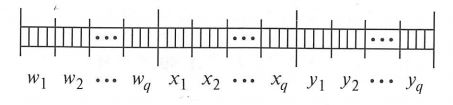
\includegraphics{figura1}
    \caption{Etiquetado de las 3q zonas, cada una contiene \(p= \ceil \lg (k+1) \ceil\) bits de representación binaria para $s(a)$, usada para transformar \lgs{3dm} en \gls{part}.}
    \label{fig:my_label}
\end{figure}
\par 

La representación para $s(a)$ depende de la correspondiente tripleta $m_i = (w_{f(i)}, x_{g(i)}, y_{h(i)} )\in M)$ (donde f, g y h son solo funciones que dan los subíndices del primer, segundo y tercer componente para cada $m_i$). \par 
Tiene un 1 en la posición del extremo derecho de las zonas etiquetadas por $w_{f(i)}, x_{g(i)}$ y $y_{h(i)}$ y 0's en el resto. Alternativamente, podemos escribir: \par 

\[s(a) = 2^{p(3q-f(i))} + 2^{p(2q-g(i))} + 2^{p(q-h(i))}\]

Dado que cada $s(a_i)$ puede ser representado como un número binario con no más de \textit{3pq} bits, esta claro que $s(a_i)$ puede ser construido desde la instancia 3DM en tiempo polinomial. \par 

Lo importante es observar en esta parte de la construcción es que, si sumamos todas las entradas de cada zonas, para todos los elementos \({a_i:\leg i\leq k}\), el total nunca superará \(k=2^p-1\). Por lo tanto, al sumar \(\sum_{a \in A'}^{} s(a)\) para cada subconjunto \(A'\subseteq\{a_i:\leg i\leq k\}\) satisfacerá

\[\sum_{a \in A'}^{} s(a) = B\]

sí y sólo sí \(M'= \{m_i:a_i\in A'\}\) es un emparejamiento para M. \par 
El paso final de la construcción especifica los dos últimos elementos de A. Estos son denotados por $b_1$ y $b_2$ y tienen tamaños definidos por

\[s(b_1) = 2 \Big[\sum_{i=1}^{k} s(a_i)\Big] - B\]
y
\[s(b_1) = 2 \Big[\sum_{i=1}^{k} s(a_i)\Big] + B\]
\newpage

Ambas pueden ser representadas en binario con no más de \((3pq+1)\) bits y así pueden ser construidas en tiempo polinomial en el tamaño de la instancia dada del problema \gls{3dm}. \par 

Ahora supon que tenemos un subconjunto \(A'\subseteq A\) tal que

\[\sum_{a \in A'}^{} s(a) = \sum_{a \in A-A'}^{} s(a)\]
Entonces ambas de estas sumas serán igual a \(2\sum_{i=1}^{k} s(a_i)\), y uno de los dos conjuntos, A' o A-A', contiene $b_1$ pero no $b_2$. El elemento restante del conjunto formado por el subconjunto de \({a_i:\leg i\leq k}\) cuyos tamaños suman B, y por lo tanto, por nuestros comentarios anteriores, este subconjunto corresponde al emparejamiento M' y M. Al contrario, si \(M'\subseteq M\) es un emparejamiento, entonces el conjunto \(\{b_1\} \cup \{a_i:m_i\in M'\}\) forma el deseado conjunto A' para la instancia de \gls{part}. \par

Por lo tanto, \(\gls{3dm} \alpha \gls{part}\), y se prueba así la $\mathcal{NP}$-completitud.

\end{proof}

\printglossary[type=\acronymtype]

\end{document}
